% sections/theory.tex: Section 4: the model, the sufficient-statistic results with the two provisos, and the mapping from
% responses to a rate. Proofs in Appendix appendix:multiperiod; the two-period derivation in Appendix appendix:proofs.
\section{A Sufficient Statistics Approach to Measuring Discount Rates}\label{sec:suffstats}

\paragraph{Notation.} Throughout the paper $\delta$ is the exponential discount factor, $\beta$ the present-bias parameter of the quasi-hyperbolic extension (Appendix \ref{appendix:nonclassical}), which equals one under exponential discounting, and $\rho$ the continuous annual discount rate ($\delta = e^{-\rho}$ over a year and $e^{-\rho/12}$ over a month); the persistence of income in the calibration appendix is $\varrho$. $D(k)$ is the discount function, the weight on utility $k$ periods ahead, with $D(0) = 1$ and $D(k) = \delta^k$ under exponential discounting. $\lambda$ is the marginal-utility ratio of equation \eqref{eq:twoperiod}: the expected marginal utility of a dollar to a borrower who is still repaying at a later date, divided by the marginal utility of a dollar to the borrower who is exactly indifferent between paying and defaulting today. $\gamma$ is relative risk aversion; regression coefficients have subscripts ($\gamma_m$, $\gamma_T$); the loss-aversion coefficient of the reference-dependent extension is $\lambda_L$ and $\theta_s$ the attention weight of the same extensions (Appendix \ref{appendix:nonclassical}). $\sigma$ is the default penalty flow of the $T$-period model, $\kappa_B$ the scale of the penalty that rises with the balance owed, and $h$ the annual hazard at which a loan ends before maturity for a reason other than default. No functional form for utility enters the identifying identity; functional forms are used in two places only, the calibration that makes $\lambda$ a function of a group's default rate (Appendix \ref{appendix:mucorrection}) and the simulated model of Appendix \ref{appendix:mcliquidity} that analyzes how sensitive the rate is to the option to default later.

What can we learn about households' impatience from their default decisions? The rate at which a household borrows reveals a composite of its discount rate, its subjective probability of repaying and the premium on a present dollar, and does not point-identify the discount factor (Appendix \ref{appendix:beliefs}). Default decisions encode a richer intertemporal tradeoff. I show that in a simple endogenous default model with separable utility, the causal effects on default of changes in repayment obligations at two different time horizons are sufficient to point-identify the discount factor $\delta$ between those two horizons, up to a single marginal-utility ratio, which the experiments of Section \ref{sec:quasi} measure and Appendix \ref{appendix:mucorrection} bounds from the persistence of the marginal borrower's economic state. No functional form for the utility function is required beyond strict concavity and monotonicity for the identifying identity itself.

The economic intuition is as follows. An impatient borrower responds to the payment due now and little to the same dollars due later: a higher payment this month raises the temptation to default, and a higher payment a year from now barely moves it. A patient borrower responds to a dollar due later nearly as she responds to a dollar due now. The ratio of the response to a later payment to the response to the current one reveals the weight the borrower places on the future relative to the present. The contract's length is not that comparison. A longer contract at a fixed payment adds payments at the far end, but it also raises the balance the lender can pursue after default and the number of months in which a default can occur (Proposition \ref{prop:termmargin}).

Can default choices reveal time preferences? The theory's answer is yes, with two provisos. First, the payment due now has a premium over every later payment, the marginal-utility ratio $\lambda$, which multiplies the discount function; no comparison of a payment due now with payments due later, in any experiment, separates that premium from present bias, because the two enter every default response as a product (Theorem \ref{thm:betalambda}). A comparison of a liquid with an illiquid dollar at one date does separate them (Corollary \ref{cor:separate}); the paper measures the premium from one such comparison, Indarte's, and Section \ref{sec:quasi} reports how much the rate moves with it. Second, beliefs enter the same weights as a product with the discount function: the borrower's own probability of still facing a payment, and her expectation of her income at the date the payment is due (Proposition \ref{prop:beliefs}). The discount function is identified with beliefs fixed; the panel fixes survival at its measured value, and Appendix \ref{appendix:beliefs} sizes both beliefs in the Survey of Consumer Finances, which is what that survey is for in this paper. The contract's length, the bureau's own source of variation in far payments, is not a payment at a date, and what it measures is stated where it is used (Section \ref{sec:identification}, Proposition \ref{prop:termmargin}). Variation that moves a payment at a known date with the balance fixed, the rule-based experiments, identifies a rate without a model of the penalty; run over outcome windows of years at horizons of four to twenty-six years, the published experiments accept the bureau's estimate and reject little else, for the reason Section \ref{sec:mapping} gives, and they check the sign and the horizon of the far-payment response rather than its level. Section \ref{sec:model} sets out the model, Section \ref{sec:results} states the identity and the two results, with proofs in Appendix \ref{appendix:multiperiod}, Section \ref{sec:mapping} maps default responses to a rate, and Section \ref{sec:quasi} applies the mapping to the rule-based experiments.

\subsection{The Model}\label{sec:model}

\paragraph{Two periods.} Payments are due at two dates, $m$ now and $L - m$ later, with $L = 2m$ in the base case. Income $y_1$ is drawn from a distribution $F$ and is net of the household's non-discretionary expenses throughout the paper, so that a shock to $y$ is an expense shock as much as an earnings shock \citep{fulford_expense_2024}; no distributional assumption is needed. Default costs a punishment $\sigma$, which stands for credit-market exclusion, stigma and garnishment \citep{indarte_moral_2023}, and the borrower has strictly increasing, strictly concave utility, additive across the two dates with discount factor $\delta$. The date-2 threshold $y_2^*$ equates the utility of paying with the utility of defaulting, and the date-1 threshold $y_1^*$ equates the value of paying now, $u(y_1 - m) + \delta\,\mathbb{E}[V_2^P]$, with the value of defaulting now, $u(y_1) + \delta\,\mathbb{E}[V_2^N]$, where $V_2^P$ and $V_2^N$ are the date-2 values after paying and after defaulting (Appendix \ref{appendix:proofs} states the problem in full):
\begin{equation}\label{eq:threshold1}
u(y_2^* - (L - m)) = u(y_2^*) - \sigma, \qquad u(y_1^* - m) + \delta\,\mathbb{E}[V_2^P] = u(y_1^*) + \delta\,\mathbb{E}[V_2^N].
\end{equation}
Default probabilities are $p_t = F(y_t^*)$, and implicit differentiation of the date-1 condition gives the two responses that everything else is built on (Appendix \ref{appendix:proofs}):
\begin{equation}\label{eq:sensitivities}
\frac{\partial p_1}{\partial L} = f(y_1^*)\,\delta\,(1 - p_2)\,\frac{\mathbb{E}\left[u'(C_2^P) \mid y_2 > y_2^*\right]}{u'(y_1^* - m) - u'(y_1^*)}, \qquad
\frac{\partial p_1}{\partial m} = f(y_1^*)\,\frac{u'(y_1^* - m)}{u'(y_1^* - m) - u'(y_1^*)} - \frac{\partial p_1}{\partial L},
\end{equation}
with $C_2^P = y_2 - (L - m)$ the consumption of a date-2 repayer. A higher far payment $L$ lowers the continuation value of repaying and raises default; a higher current payment $m$ raises the marginal utility of consuming today and the gain from not paying. The ratio of the two responses eliminates the density at the default margin and the scale of utility. Write $A \equiv \partial p_1/\partial L$ for the response to the far payment and $B \equiv (1 - p_2)\,\partial p_1/\partial m$ for the response to the current payment, scaled by the probability of reaching the second date. Then
\begin{equation}\label{eq:twoperiod}
\frac{A}{A + B} \;=\; \delta\,\lambda, \qquad
\lambda \;\equiv\; \frac{\mathbb{E}\left[u'(C_2^P) \mid y_2 > y_2^*,\, y_1 = y_1^*\right]}{u'(y_1^* - m)}.
\end{equation}
The left side is the share of the total default response that the far payment accounts for. The right side is the discount factor times the \emph{marginal-utility ratio} $\lambda$, defined in the same display: the average marginal utility of future repayers conditional on standing at today's default margin, over the marginal utility of the marginal defaulter herself. With concave utility they differ, and for a liquidity-constrained borrower the ratio is well below one. If default decisions are entirely forward-looking, the far payment accounts for the whole response and $\delta\lambda = 1$; if they are entirely myopic, $\delta\lambda = 0$. The two-period model offers one future date and identifies the product $\delta\lambda$, not its factors; the $T$-period model below offers many, and two future dates $t_1, t_2 \ge 2$ identify $\delta$ alone:
\begin{equation}\label{eq:twofuture}
\frac{\partial p_1/\partial m_{t_2}}{\partial p_1/\partial m_{t_1}} \;=\; \delta^{\,t_2 - t_1}\,\frac{Q_{t_2}}{Q_{t_1}},
\end{equation}
where $Q_t$ is the probability of still facing the payment at $t$, when the marginal-utility ratio is the same at the two dates; in general the ratio has the further factor $\lambda_{t_2}/\lambda_{t_1}$, which the profile stated below supplies. This is the comparative static the abstract names, and the two-arm experiments of Section \ref{sec:quasi} supply it. The paper treats $\lambda$ as a measured input rather than an assumption: Section \ref{sec:quasi} measures it from the pair of responses in \citet{indarte_moral_2023}, to a dollar of payment relief within the year and to a dollar of seizable wealth at the filing date, which compares a liquid dollar with an illiquid one for a household at the bankruptcy margin, at $\lambda \approx 0.2$; Appendix \ref{appendix:mucorrection} bounds it from the other side, from the measured persistence of the distress state (Table \ref{tab:mucorrection}). The comparisons of payment elasticities in Section \ref{sec:heterogeneity} do not involve $\lambda$, and the rate comparisons of Section \ref{sec:rate_people} use each group's own profile; the level of the rate depends on how the premium is spread over the later payments, and Sections \ref{sec:quasi} and \ref{sec:rate_people} report the sensitivity.

\paragraph{$T$ periods.} The two-period structure is a special case of a general model. A contract specifies payments $m_t > 0$ at dates $t = 1, \dots, T$, with balance $L = \sum_t m_t$; for an annuity, $m_t = m$ at every date. Income $y_t$ is drawn i.i.d.\ from $F$ with continuous density $f$ and full support on $(0,\infty)$; the results below go through with Markov income (Remark \ref{appendix:continuous} in Appendix \ref{appendix:multiperiod}); income is net of non-discretionary expenses throughout. Consumption equals income net of any payment, utility $u$ is strictly increasing, strictly concave, and satisfies $u(0^+) = -\infty$ (e.g.\ CRRA with $\gamma \ge 1$). Default is absorbing: a borrower who defaults at $t$ consumes her income thereafter and incurs a punishment flow $\sigma > 0$ in each period $s \in \{t, \dots, T\}$; Section \ref{sec:results} adds a component of the punishment that scales with the balance owed. All agents are identical after $T$, so post-$T$ values are normalized to zero. The borrower discounts utility $k$ periods ahead by the discount function $D(k)$, exponential, $D(k) = \delta^k$, unless stated otherwise. A loan may also end before the next payment for a reason other than default, with monthly probability $1 - e^{-h/12}$ at the annual exit hazard $h$: the borrower sells or trades in the vehicle and pays the loan off, refinances it, or the loan is transferred to another servicer, which ends it under one furnisher's key and restarts it under another's (Appendix \ref{appendix:data}). The results are stated with $Q_s$ the probability that the borrower still faces the payment at $s$, which the exits lower, and Section \ref{sec:mapping} states how it is measured.

Let $W_t = \sum_{k=0}^{T-t}\delta^k(\mathbb{E}u(y) - \sigma)$ denote the defaulted value and
\begin{equation}\label{eq:bellmanT}
V_t(y) = \max\big\{\, u(y - m_t) + \delta \mathbb{E}V_{t+1},\;\; u(y) - \sigma + \delta W_{t+1} \,\big\}, \qquad V_{T+1} \equiv 0,
\end{equation}
the value of good standing. Write the surplus from staying as $\Delta_t(y) = K_t - g_t(y)$, where $g_t(y) \equiv u(y) - u(y-m_t) > 0$ is the utility cost of paying, strictly decreasing on $(m_t,\infty)$, and $K_t \equiv \sigma + \delta(\mathbb{E}V_{t+1} - W_{t+1})$ is the value of standing. The borrower defaults iff $y < y_t^* = g_t^{-1}(K_t)$, so that $p_t = F(y_t^*)$, and $Q_s = \prod_{k=2}^{s}(1-p_k)$ is the probability of good standing through date $s$. Default is an optimal stopping problem: a borrower who stays today is not committing to repay the remaining $T-t$ installments but buys one period of good standing plus the option to reconsider, and Proposition \ref{prop:interiorT} in Appendix \ref{appendix:multiperiod} shows that, for this reason, every default probability is strictly interior at any horizon $T$ and any payment schedule, provided the punishment has a flow component. The same appendix characterizes the two modeling choices that instead produce degenerate corner probabilities, comparing default against committed repayment of all remaining installments (Lemma \ref{lem:committedT}) and letting the punishment vanish at maturity.

\paragraph{The marginal-utility ratio with many dates.} With many dates the ratio is date-specific: $\lambda_s = \mathbb{E}[u'(y - m_s) \mid y > y_s^*]/u'(y_1^* - m_1)$ compares the repayers' expected marginal utility at $s$ with the marginal defaulter's today. With income independent across months and a constant payment, the repayers' expected marginal utility is the same at every future date, so $\lambda_s = \lambda$ for all $s \ge 2$: the two-period object applied to every later payment, the convention under which Indarte's pair is mapped to $\lambda$. With a persistent income state the profile declines: a borrower at the default margin today is likely still constrained next month, so $\lambda_2$ is near one, and $\lambda_s$ falls toward the independent-income value as the distress state mean-reverts. The paper maps every ratio through the profile, because the profile is the measured object: the persistence of the distress state is measured in the panel, $0.52$ per year (Appendix \ref{appendix:measuredrho}), and the curvature that turns persistence into a profile is the one that passes the constant-income limit through Indarte's value. Under that persistence the calibration that gives $\lambda(p) = 0.34$ for the pooled auto population as a constant gives $\lambda_2 = 0.89$, $\lambda_{12} = 0.59$ and $\lambda_{60} = 0.35$ (equation \eqref{eq:lambda_p}). A declining profile gives the near payments more weight than a constant assigns them, so that for a given ratio of the far-payment response to the payment response a constant premium returns a rate above the profile's; Section \ref{sec:rate_people} reports the constant-premium rate beside the estimate as the sensitivity.

\subsection{Sufficient-Statistic Results}\label{sec:results}

Fix the schedule $(m_1,\dots,m_T)$ and let $\Delta u_1' \equiv u'(y_1^* - m_1) - u'(y_1^*) > 0$ denote the gap in marginal utility across the two branches at the date-1 threshold. Appendix \ref{appendix:multiperiod} proves each result of this subsection.

\begin{proposition}[Sensitivities to the payment schedule]\label{prop:sensT}
Under exponential discounting,
\begin{align}
\frac{\partial p_1}{\partial m_1} &= f(y_1^*)\,\frac{u'(y_1^* - m_1)}{\Delta u_1'}, \label{eq:sens1T}\\
\frac{\partial p_1}{\partial m_s} &= f(y_1^*)\,\delta^{s-1} Q_s\, \frac{\mathbb{E}[u'(y - m_s) \mid y > y_s^*]}{\Delta u_1'}, \qquad s \ge 2, \label{eq:senssT}
\end{align}
where $Q_s = \prod_{k=2}^{s}(1-p_k)$ is the probability of good standing through date $s$.
\end{proposition}

With $T = 2$, $m_1 = m$, and $m_2 = L - m$, equations \eqref{eq:sens1T}--\eqref{eq:senssT} reduce exactly to equation \eqref{eq:sensitivities}. The ratio of the response to a later payment to the response to the current one cancels the density at the default margin and the scale of utility. Under a general discount function $D$, with either exponential discounting or a naive borrower, the same argument gives
\begin{equation}\label{eq:curveT}
\frac{\partial p_1/\partial m_s}{\partial p_1/\partial m_1} = D(s-1)\, Q_s\, \frac{\mathbb{E}[u'(y-m_s) \mid y > y_s^*]}{u'(y_1^* - m_1)}, \qquad s = 1, \dots, T.
\end{equation}
The right side is the weight a payment due at $s$ has relative to the payment due now,
\begin{equation}\label{eq:weights}
w_1 = 1, \qquad w_s = D(s-1)\,Q_s\,\lambda_s, \qquad \lambda_s \equiv \frac{\mathbb{E}[u'(y - m_s) \mid y > y_s^*]}{u'(y_1^* - m_1)}, \qquad s \ge 2,
\end{equation}
the product of the discount function, the probability of still facing the payment, and the marginal utility of a dollar at $s$ relative to a dollar at today's default threshold. In logs the weight is the Euler equation's decomposition of the rate a household demands to defer a dollar: $-\log w_s = \rho\,(s-1)/12 - \log\lambda_s - \log Q_s$, pure impatience plus a consumption-smoothing term plus survival. A household at the default margin may weigh a later dollar lightly not because it is impatient but because it expects its own circumstances to improve, the borrower who sees herself as temporarily embarrassed; that expectation is the consumption-smoothing term, and it is $\lambda_s$, measured, and not $\rho$. The identification results below are statements about which comparisons move which term. A treatment that changes the payment path by $\{X_s\}$ therefore moves default by $\phi\sum_s w_s X_s$ to first order, with the scale $\phi = f(y_1^*)\,u'(y_1^* - m_1)/\Delta u_1'$ common to every date, and the ratio of two treatments' effects in the same population is the ratio of their weighted sums, in which $\phi$ cancels. This is the identity every estimate in the paper is built on; it identifies $D$ given survival and the marginal-utility ratio. Every outcome in the paper is measured within a window, default within $K$ months, and a window aggregates decisions: a loan that defaults in month $t$ of the window did so at a decision at which the payment due now was the $t$-th and the far payments stood $T - t$ months ahead. With $\omega_t$ the share of the window's defaults that occur in month $t$, measured in the panel, the response of default within the window to a treatment is $\phi\sum_{t \le K}\omega_t\sum_{s \ge t} w^{(t)}_{s-t+1} X_s$, with $w^{(t)}$ the weights of equation \eqref{eq:weights} taken from the decision date $t$. For an annuity of $T$ payments under exponential discounting and survival at the exit hazard $h$, the elasticity of default within $K$ months to the contract's length at a fixed payment, which adds a payment at the end of the contract, over its elasticity to the payment, which moves every payment, is to first order
\begin{equation}\label{eq:window}
R_K \;=\; \frac{\sum_{t \le K}\omega_t\, T\, w_{T-t+1}}{\sum_{t \le K}\omega_t \sum_{k=1}^{T-t+1} w_k}, \qquad w_1 = 1, \qquad w_k = \lambda_k\,e^{-(\rho + h)(k-1)/12}, \quad k \ge 2,
\end{equation}
the formula through which Section \ref{sec:rate_people} maps the bureau's within-borrower ratios to a rate and Section \ref{sec:quasi} tests the experiments' pairs, each with its own window and event timing in place of $\omega_t$. With $K = 1$ and a constant $\lambda_k = \lambda$ it is the date-1 formula $R = T w_T/\sum_{s \le T} w_s$ of a decision at origination, the special case without a balance-scaled penalty of equation \eqref{eq:Rs} in Appendix \ref{appendix:formula}. The date-1 formula assigns every default in a two-year window to a decision at origination, where the far payment is farthest and its weight smallest; a default in month 24 was decided when the far payment stood 37 months ahead rather than 60, and the date-1 formula reads the same ratio as a lower rate than the window's decisions reveal.

The two provisos follow from equation \eqref{eq:curveT}. The first concerns the weight on the payment due now.

\begin{proposition}[The present-payment premium]\label{prop:premium}
In the model of Proposition \ref{prop:sensT}, the weight on the payment due now relative to the payment due at $s \ge 2$ is
\[
\frac{\partial p_1/\partial m_1}{\partial p_1/\partial m_s} \;=\; \frac{1}{D(s-1)\,Q_s\,\lambda_s},
\]
with $\lambda_s$ the marginal-utility ratio of equation \eqref{eq:weights}, and $\lambda_s < 1$ whenever the marginal defaulter's consumption at date 1, $y_1^* - m_1$, is below the repayers' expected consumption at date $s$. The present payment therefore has a premium over every later payment that is separate from, and multiplies, the discount function, and it is bounded away from one for a liquidity-constrained marginal defaulter however patient she is.
\end{proposition}

\begin{theorem}[Present bias and the premium are not separable]\label{thm:betalambda}
Let $D(k) = \beta\delta^k$ for $k \ge 1$ with $D(0) = 1$, and let $\lambda_s = \lambda$ for all $s \ge 2$. Then every ratio of default responses to payments at dates $s, s' \ge 1$ depends on $(\beta, \lambda)$ only through the product $\beta\lambda$: for $s \ge 2$, $(\partial p_1/\partial m_s)/(\partial p_1/\partial m_1) = \beta\lambda\,\delta^{s-1} Q_s$, and for $s, s' \ge 2$ the ratio is $\delta^{s-s'} Q_s/Q_{s'}$. Consequently no set of perturbations of the payment schedule, however rich, and no experiment that moves payments due now against payments due later, identifies $\beta$ and $\lambda$ separately; $\delta$ and the product $\beta\lambda$ are identified, and $\beta = 1$ is observationally equivalent to any $(\beta, \lambda')$ with $\beta\lambda' = \lambda$.
\end{theorem}

\noindent The present-bias parameter of \citet{laibson_golden_1997} and the marginal-utility ratio that \citet{indarte_moral_2023} conditions on distress are, in every model of this class, the same object as far as default responses to payment timing are concerned: they enter every such response only as the product $\beta\lambda$. A study that attributes the whole premium to present bias measures its $\beta$ as this paper's $\lambda$, and one that attributes it wholly to liquidity measures its $\lambda$ as the other's $\beta$.

\begin{corollary}[What separates them]\label{cor:separate}
$\lambda$ is identified by a comparison at one date between a dollar valued at the marginal defaulter's marginal utility and a dollar valued at a repayer's: a change in liquid resources at the decision date against a change in the value of default at the same date, such as the payment-reduction and seizable-equity responses of \citet{indarte_moral_2023}, whose ratio does not depend on $D$ except through the months over which the relief is spread. The ratio equals $\lambda$ under the assumption that the marginal utility of a dollar of protected, illiquid wealth to a household at the default margin is the marginal utility of a repayer's later dollar, which is the sense in which both are the price of liquidity at the margin. Given $\lambda$, the product identifies $\beta$. Absent such a pair, a reader may attribute the whole premium to present bias or the whole of it to liquidity; the data cannot adjudicate, and the paper reports the product as one measured number.
\end{corollary}

The second proviso concerns the survival weight.

\begin{proposition}[Beliefs enter the weights multiplicatively]\label{prop:beliefs}
Let the borrower's subjective probability of remaining in good standing through $s$ be $\tilde Q_s$, possibly different from the objective $Q_s$. Then \eqref{eq:curveT} holds with $\tilde Q_s$ in place of $Q_s$, and the object identified from default responses with objective survival substituted is $D(s-1)\,\tilde Q_s/Q_s$. The discount function is identified only with beliefs fixed, and fixing them at the objective survival measured in the panel loads any optimism or pessimism about survival onto $D$.
\end{proposition}

\noindent This is the non-identification of \citet{manski_measuring_2004}, that choices reveal preferences only jointly with beliefs, in the setting of default responses: subjective and objective survival cannot be told apart from the responses alone. The paper's response is to measure $Q_s$ directly, from the exit, default and cure hazards of the panel, to state every discount rate as the rate that rationalizes the observed responses under those beliefs, and to size in survey data how far the beliefs of constrained households depart from the objective values (Appendix \ref{appendix:beliefs}). The expectation of income at the date a payment is due enters the same way, through $\lambda_s$.

Three further results of Appendix \ref{appendix:multiperiod} are used later. Proposition \ref{prop:curveT} states what an experiment must do to identify the whole discount curve: perturb each payment separately within one population, and with three or more future horizons the exponential form is testable; Remark \ref{rem:experimentsT} states why comparisons across borrowers who selected into different contract lengths do not qualify. Remark \ref{rem:option} states that a borrower who continues keeps the option to default later, so the far payments enter her decision only with the weight of the states in which she will still be paying them; for that reason the decline of the payment response with loan age is compared with the stopping model's own decline rather than mapped to a rate (Section \ref{sec:mainresults}, Appendix \ref{appendix:mcliquidity}).

\subsection{From Default Responses to a Discount Rate}\label{sec:mapping}

Proposition \ref{prop:sensT} gives the default response to a change in the payment at date $s$ as the product of a common scale $\phi$ and the date-specific weight of equation \eqref{eq:weights}, and the ratio of two treatments' effects in the same population cancels the scale. The ratio identifies the discount function only with the other two weights, survival and the marginal-utility ratio, supplied, and this subsection states how each is.

Survival is measured. For a borrower deciding today, $Q_s$ is the probability of being current at $s$, which falls with the default hazard and the payoff hazard. In the model default is absorbing, the terminal event that ends the contract; in the data a delinquency spell that begins does not always end the contract, since one fifth of delinquent auto trades return to current within a four-month interval (Appendix \ref{appendix:measuredrho}). The cure rate therefore scales the delinquency hazard to the hazard of the terminal event the model describes. For the experiments of Section \ref{sec:quasi} the default and payoff hazards are each study's own, and the cure rate is the one bureau input; for the auto-loan panel Section \ref{sec:autodata} measures the default and payoff hazards directly.

The marginal-utility weight $\lambda_s$ is the ratio of the average repayer's marginal utility at $s$ to that of the marginal defaulter today, below one when the marginal defaulter is liquidity-constrained (Proposition \ref{prop:premium}), and it is a profile over the horizon, from one source. Its level is measured: $0.2$ is the value that the comparison of a payment reduction with a change in seizable home equity in \citet{indarte_moral_2023} identifies under the assumption of Corollary \ref{cor:separate}, at her population's default rate and payment share (Section \ref{sec:quasi}). Its dependence on the group is the function $\lambda(p)$ of the default rate, the constant-relative-risk-aversion calibration of Appendix \ref{appendix:mucorrection} that passes through Indarte's value: a group whose default is rare has its marginal defaulter far in the lower tail of income, where marginal utility is steep, and therefore a smaller weight. Its shape over the horizon is the profile of Section \ref{sec:model} at the persistence of the distress state measured in the panel, equation \eqref{eq:lambda_p}: across the bureau's groups $\lambda_2$ is $0.88$ to $0.89$ and $\lambda_{60}$ runs from $0.26$ to $0.40$, and for each experiment's population the profile is taken at the study's own baseline rate and payment share. Sections \ref{sec:quasi} and \ref{sec:rate_people} report how far the estimates move under a constant premium of $0.2$ or $0.5$ in place of the profile.

For the credit-bureau data there is one more step. The term margin contains the penalty channel of Proposition \ref{prop:termmargin}, whose weight on a distant payment is $\kappa_B(1+r)^{-(s-1)}$ at the contract rate $r$, and, across borrowers, selection into contract length. Within borrower, selection is removed by design; the estimate of Section \ref{sec:rate_people} is taken at twenty-four months, where the penalty channel, which dominates within the first year, has decayed with the balance, and the deficiency contrast of Section \ref{sec:termmargin} measures the size of that channel. Across borrowers the two channels are adjusted for one at a time in Appendix \ref{appendix:ladder}, which reproduces the within-borrower estimate with less precision. The decline of the payment response with loan age is compared with the stopping model's own decline rather than mapped to a rate, for the reason Remark \ref{rem:option} gives. The rule-based experiments, which move payments by rule and hold the balance's legal treatment fixed, identify a rate without a model of the penalty; the next paragraph states why, at the windows and horizons at which they were run, they check the sign and the horizon of the far-payment response and not its level.

Figure \ref{fig:design_map} in Appendix \ref{appendix:figures} shows how the designs of the paper, each in its own section, supply the inputs of the formula and what each output rests on.

\paragraph{The horizon at which a rate can be estimated.} The weights say where in a contract a rate can be estimated and where it cannot. A response to a payment at horizon $s$ estimates the weight $w_s = \lambda e^{-(\rho + h)(s-1)/12}$ with some sampling error, and the rate is obtained from the weight's dependence on $\rho$. The delta method gives the standard error of the rate as the standard error of the response over $|\partial w_s/\partial \rho| = (s-1) w_s/12$, so that, for a response measured with a given absolute precision, the standard error of $\rho$ is proportional to $e^{(\rho + h)(s-1)/12}/(s-1)$. Compounding makes a far weight more sensitive to the rate, in proportion to the horizon; discounting and survival make the weight itself, and with it the response the data contain, smaller, exponentially in the horizon. The standard error is smallest at a horizon of $1/(\rho + h)$ years, $3.3$ years at the rate and exit hazard of the auto panel, and rises without bound on either side: at 26 years, the horizon of the Ganong--Noel forgiveness arm, $134$ times less precisely (Figure \ref{fig:horizon_power}, left). The same calculation for the bureau's term-to-payment ratio of equation \eqref{eq:window}, at the precision the within-borrower design attains, gives the smallest difference in the rate that a contract of each length can detect at the 95 percent level: $0.05$ for a five-year contract in one score decile, $0.06$ for a ten-year contract, and $2.4$ for a thirty-year mortgage (Figure \ref{fig:horizon_power}, right). A window adds a second loss. An outcome measured over five years, as the Dobbie--Song pair's is, averages the far payment's weight over decisions spread across sixty months, at some of which the forgiven payments are a year away and at others four, and the averaged weight moves with the rate more slowly than any one decision's does: aggregated over its own window, the pair accepts every rate from zero to $1.2$ at the five percent level (Section \ref{sec:quasi}). No design in these data, and no published experiment, estimates a long-run rate: the paper's object is the rate over the horizon of an installment contract, the auto loan sits where that rate is best measured, and that is why the level is the bureau's and the experiments are the check.

\begin{figure}[ht]
\centering
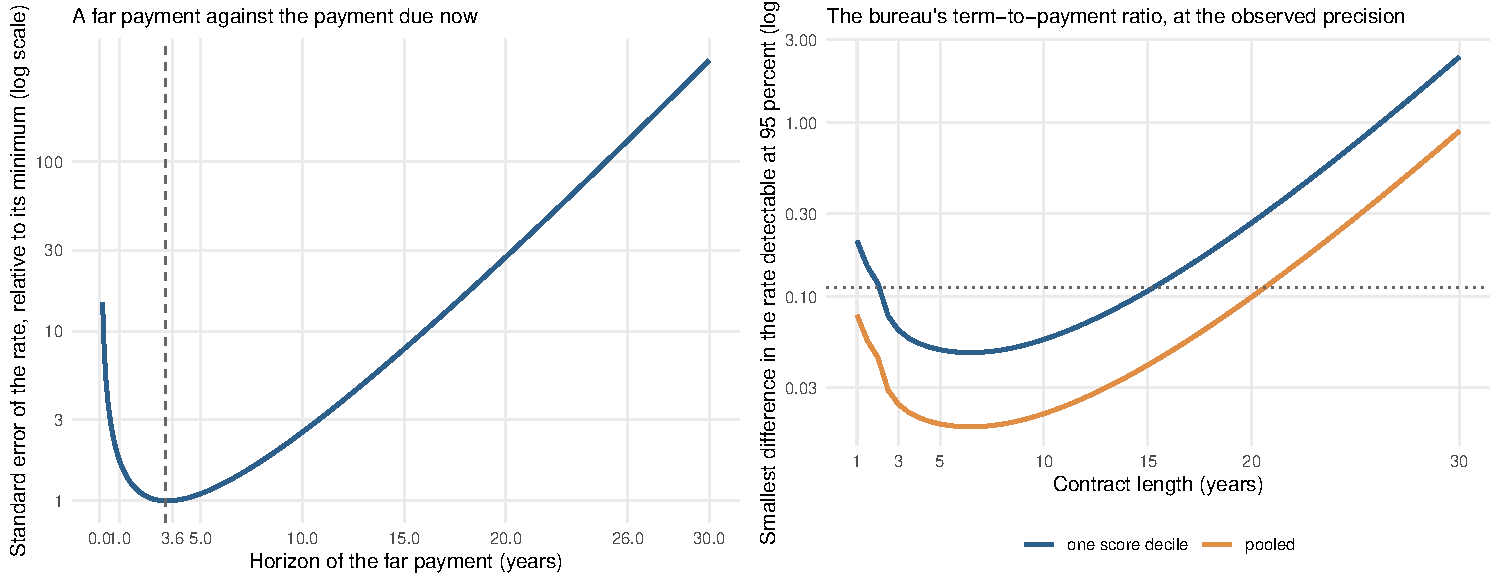
\includegraphics[width=\textwidth]{figures/fig_horizon_power.pdf}
\caption{The precision of the rate by horizon. Left: the standard error of the rate obtained from a single far payment against the payment due now, relative to its minimum, by the horizon of the far payment; the dashed line is $1/(\rho + h)$ years at $\rho = 0.11$ and $h = 0.19$. Right: the smallest difference in the rate detectable at the 95 percent level from the term-to-payment ratio of an annuity, by contract length, at the standard error of the ratio in the pooled within-borrower sample and in one score decile, through equation \eqref{eq:window}; the dotted line is the estimate, $0.11$.}
\label{fig:horizon_power}
% replication: Code/local/horizon_power.R; results/horizon_power.csv, results/rho_within_readings.csv
\end{figure}

